% This file was created with tikzplotlib v0.10.1.
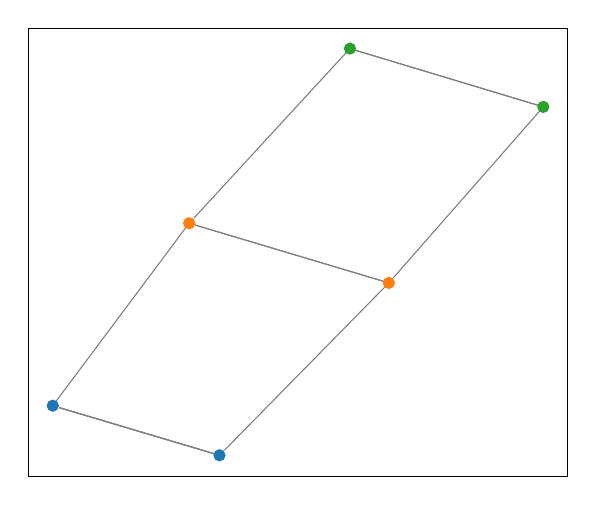
\begin{tikzpicture}

\definecolor{darkgray176}{RGB}{176,176,176}
\definecolor{gray}{RGB}{128,128,128}

\begin{axis}[
scaled x ticks=manual:{}{\pgfmathparse{#1}},
scaled y ticks=manual:{}{\pgfmathparse{#1}},
tick align=outside,
x grid style={darkgray176},
xmajorticks=false,
xmin=-0.744496262319945, xmax=0.786877453355703,
xtick style={color=black},
xticklabels={},
y grid style={darkgray176},
ymajorticks=false,
ymin=-1.08577376010661, ymax=1.09932256000508,
ytick style={color=black},
yticklabels={}
]
\draw[-,draw=gray] (axis cs:0.168452507424814,1) -- (axis cs:0.717269557188629,0.715938952189245);
\draw[-,draw=gray] (axis cs:0.168452507424814,1) -- (axis cs:0.717269557188629,0.715938952189245);
\draw[-,draw=gray] (axis cs:0.168452507424814,1) -- (axis cs:-0.287862474611815,0.1487984170015);
\draw[-,draw=gray] (axis cs:0.717269557188629,0.715938952189245) -- (axis cs:0.278863927762576,-0.142034775612619);
\draw[-,draw=gray] (axis cs:-0.67488836615287,-0.740416612087745) -- (axis cs:-0.201835151611333,-0.982285981490381);
\draw[-,draw=gray] (axis cs:-0.67488836615287,-0.740416612087745) -- (axis cs:-0.201835151611333,-0.982285981490381);
\draw[-,draw=gray] (axis cs:-0.67488836615287,-0.740416612087745) -- (axis cs:-0.201835151611333,-0.982285981490381);
\draw[-,draw=gray] (axis cs:-0.67488836615287,-0.740416612087745) -- (axis cs:-0.287862474611815,0.1487984170015);
\draw[-,draw=gray] (axis cs:-0.201835151611333,-0.982285981490381) -- (axis cs:0.278863927762576,-0.142034775612619);
\draw[-,draw=gray] (axis cs:-0.287862474611815,0.1487984170015) -- (axis cs:0.278863927762576,-0.142034775612619);
\draw[-,draw=gray] (axis cs:-0.287862474611815,0.1487984170015) -- (axis cs:0.278863927762576,-0.142034775612619);
\addplot [
  mark=*,
  only marks,
  scatter,
  scatter/@post marker code/.code={%
  \endscope
},
  scatter/@pre marker code/.code={%
  \expanded{%
  \noexpand\definecolor{thispointdrawcolor}{RGB}{\drawcolor}%
  \noexpand\definecolor{thispointfillcolor}{RGB}{\fillcolor}%
  }%
  \scope[draw=thispointdrawcolor, fill=thispointfillcolor]%
},
  visualization depends on={value \thisrow{draw} \as \drawcolor},
  visualization depends on={value \thisrow{fill} \as \fillcolor}
]
table{%
x  y  draw  fill
0.168452507424814 1 44,160,44 44,160,44
0.717269557188629 0.715938952189245 44,160,44 44,160,44
-0.67488836615287 -0.740416612087745 31,119,180 31,119,180
-0.201835151611333 -0.982285981490381 31,119,180 31,119,180
-0.287862474611815 0.1487984170015 255,127,14 255,127,14
0.278863927762576 -0.142034775612619 255,127,14 255,127,14
};
\draw (axis cs:0.168452507424814,1) node[
  scale=0.5,
  text=white,
  rotate=0.0
]{0};
\draw (axis cs:0.717269557188629,0.715938952189245) node[
  scale=0.5,
  text=white,
  rotate=0.0
]{3};
\draw (axis cs:-0.67488836615287,-0.740416612087745) node[
  scale=0.5,
  text=white,
  rotate=0.0
]{13};
\draw (axis cs:-0.201835151611333,-0.982285981490381) node[
  scale=0.5,
  text=white,
  rotate=0.0
]{14};
\draw (axis cs:-0.287862474611815,0.1487984170015) node[
  scale=0.5,
  text=white,
  rotate=0.0
]{15};
\draw (axis cs:0.278863927762576,-0.142034775612619) node[
  scale=0.5,
  text=white,
  rotate=0.0
]{16};
\end{axis}

\end{tikzpicture}
